
\section{Experimental Testbed and Platform}
%\paragraph{Grid Games}
\label{sec:grid_games}

Our experimental testbed, while still under development, already
includes several two-agent grid games.  These games are designed to
vary the level of coordination required, while at the same time
allowing agents to defend against uncooperative partners.

A grid game is a game played by two agents on a grid, in which each
agent has a goal.  See, for example, Figure~\ref{fig:hallway}, which
is a 3x5 grid in which the two agents' initial positions are one
another's goals: Orange begins in position (1,2), Blue's goal; and
Blue begins in position (5,2), Orange's goal.  We refer to grid
positions using $x$-$y$ coordinates, with $(1,1)$ as the bottom left
position.

One grid game match proceeds in rounds,
%(20, in our human experiments), 
and each round consists of multiple turns.
%(100, in our human experiments).
On each turn, the agents choose one of five actions (north, south,
east, west, or wait), which are then executed simultaneously.  In the
most basic setup, agents transition deterministically, and
there is no tie-breaking when two agents collide.%
\footnote{It is a simple matter to vary these rules within our
  infrastructure, as future experimental design might dictate.}
%
Instead, if their chosen actions would result in a collision with one
another, neither agent moves.  A round ends when either (or both)
players move into their goal, or when a maximum number of turns has
been taken.

As mentioned above, our grid games are specifically designed to
prevent the agents from reaching their goals without coordinating
their behavior.
% Consequently, if we assume
% %(as is standard)
% positive step costs, all the equilibria in our games involve mixed
% strategies (because any deterministic strategy either involves butting
% heads indefinitely, or can be exploited).  Since game theorists
% question the validity of mixed strategies as a reasonable model of
% human behavior~\cite{}, we assume zero step costs.  However, this
% assumption has the undesirable effect of rendering all strategy
% profiles in which both agents arrive at their goals simultaneously as
% equilibria, including purely cooperative strategies.
% 
% In reality, 
Consequently, one approach is for an agent to cooperate blindly with
its opponent by simply moving out of the opponent's way, and hoping
the opponent then waits for the agent to catch up.  However, such
strategies can be exploited by uncooperative ones that proceed
directly to the goal as soon as their path is unobstructed.
%(because step costs are never truly zero). 
 
To distinguish ``unsafe'' from ``safe'' cooperation, we devised a new
categorization for strategies in our grid games.  Specifically, we
call strategies that allow for cooperation, while at the same time
maintain a defensive position in the event that the other agent is
uncooperative, \mydef{cooperative defensive} strategies.  More
formally, an agent's strategy is \mydef{cooperative} (C) if it is one
that allows both it and its opponent to reach their goals, while an
agent's strategy is \mydef{defensive} (D) if its opponent does not
have a strategy that allows it to reach its goal strictly first.  A
cooperative defensive (CD) strategy is both cooperative and defensive.

We now proceed to describe a sample set of grid games, and equilibria
comprised of CD strategies (when they exist), to illustrate the kinds
of interactions we plan to study.
%
Our first example, Hallway, is depicted in Figure~\ref{fig:hallway}.
This game is one in which the agents can choose to coordinate, for
example, if both agents agree upon a joint strategy where one agent
moves along the top row and the other along the bottom, without
interfering with one another.  But, an agent could choose to ``defect''
from this joint strategy, by proceeding straight to its goal.  There
are CD strategies, however, which defend against such non-cooperative
behavior.

For example, if Orange moves south initially to $(1,3)$ and Blue moves
west to $(4,2)$, Orange might choose to return and remain on its goal
until Blue retreats to $(4,3)$ or $(4,1)$, at which point the players
are equidistant from their goals, and both can reach them safely.
This joint strategy is an equilibrium comprised of CD strategies,
since Orange and Blue both remain in positions where they have the
ability to block their opponents until they both have unobstructed
equidistant paths to their respective goals.

%Another defensive strategy for Orange from $(1,3)$ would have it
%proceed east to $(2,3)$, and then choose to move south to $(2,2)$.  If
%Blue is in $(3,2)$ and attempts to move west into $(2,2$), the agents
%would collide until one agent chooses a different action. It is in
%Orange's best interest to continue choosing south to try to take
%$(2,2)$ until Blue surrenders and chooses to go north into $(3,3)$ or
%south into $(3,1)$ to avoid further collision.  At this point, the
%agents are equidistant from their goals, and both can reach them
%safely---hence, we have another equilibrium comprised of CD strategies.

\begin{figure}
\centering
\begin{subfigure}{.3\textwidth}
\centering
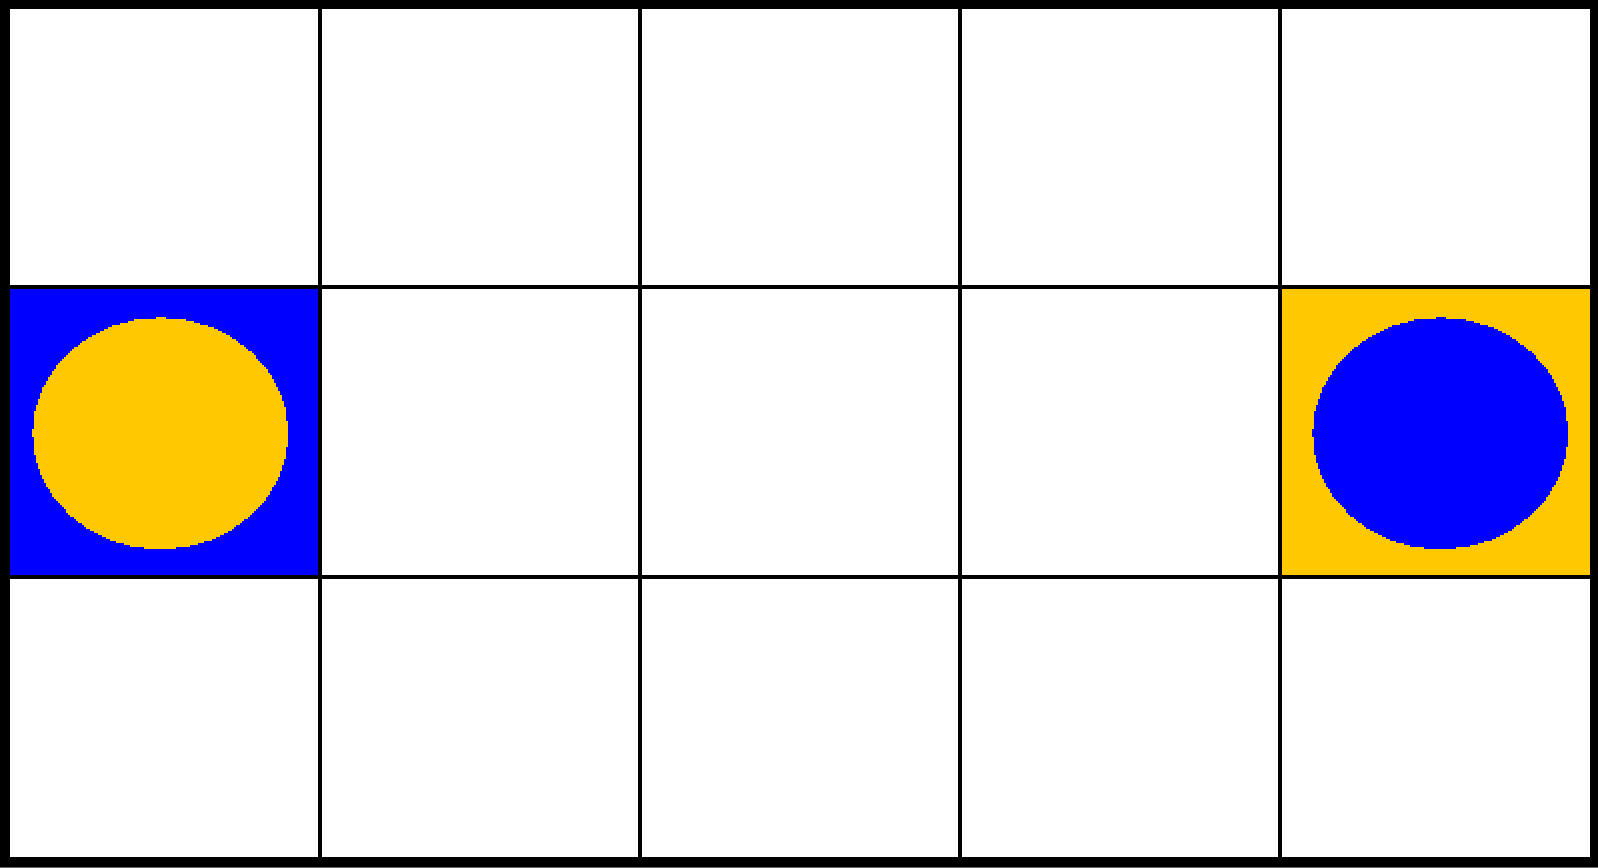
\includegraphics[width=0.65\columnwidth]{figures/threebyfive.png}
\caption{Hallway}
%\caption{Hallway, a three-by-five grid that requires a coordination strategy to efficiently play the game. Several strategies also allow an agent to defend against an uncooperative partner.}
\label{fig:hallway}
\end{subfigure}
\begin{subfigure}{.3\textwidth}
\centering
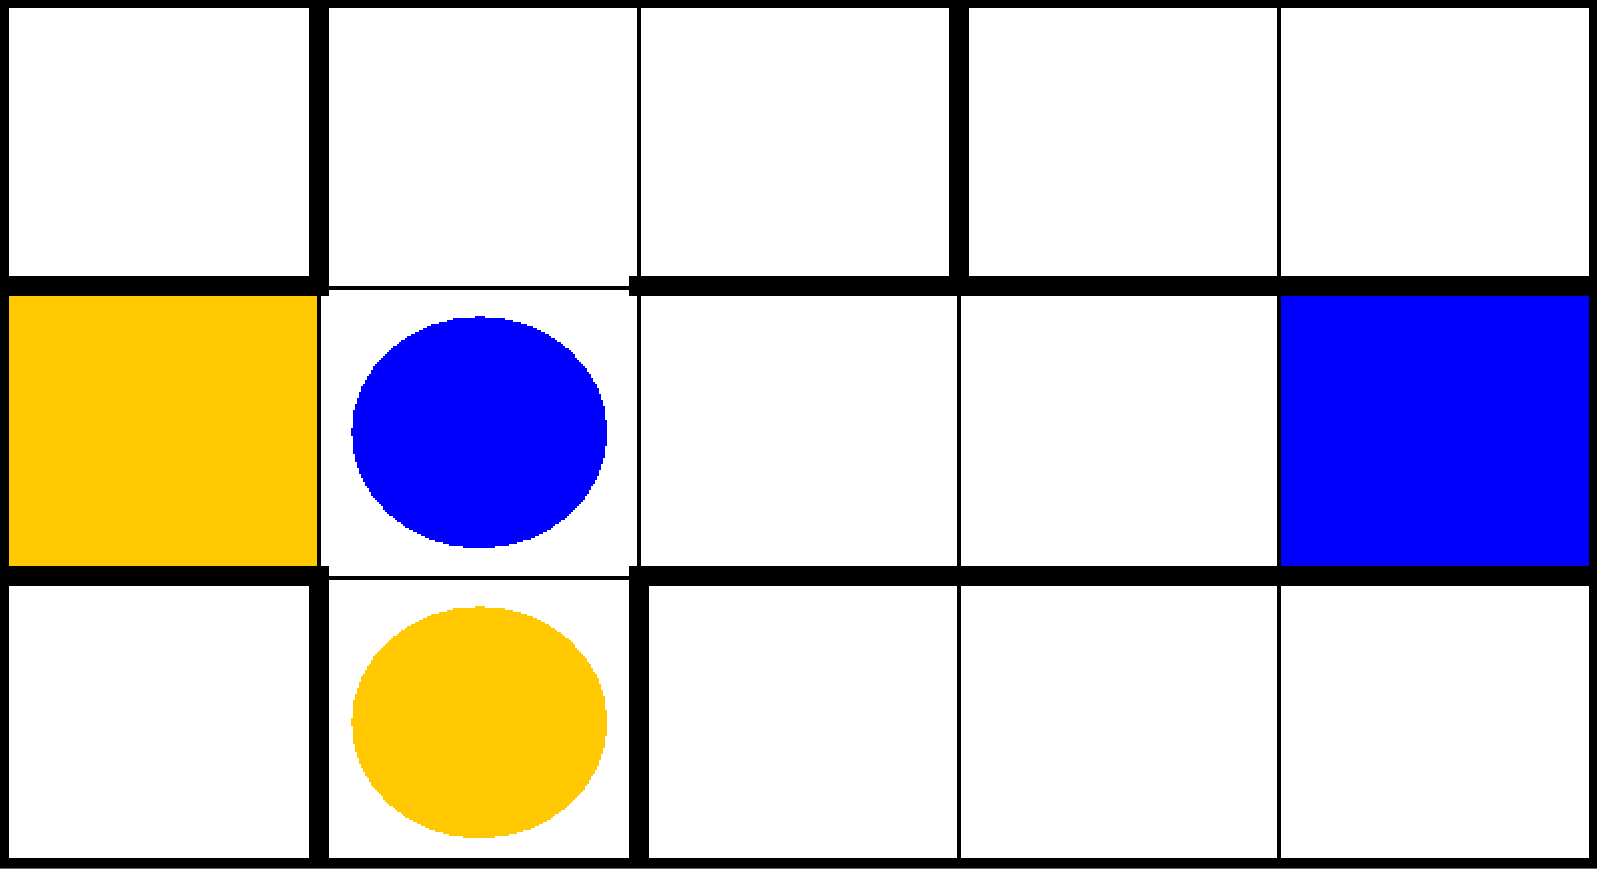
\includegraphics[width=0.65\columnwidth]{figures/threebyfivehallways.png}
%\caption{Intersection, a three-by-five grid that requires Blue to defend Orange's goal to encourage Orange to cooperate and move to the end of the uppermost hallway.}
\caption{Intersection}
\label{fig:intersection}
\end{subfigure}
\begin{subfigure}{.3\textwidth}
\centering
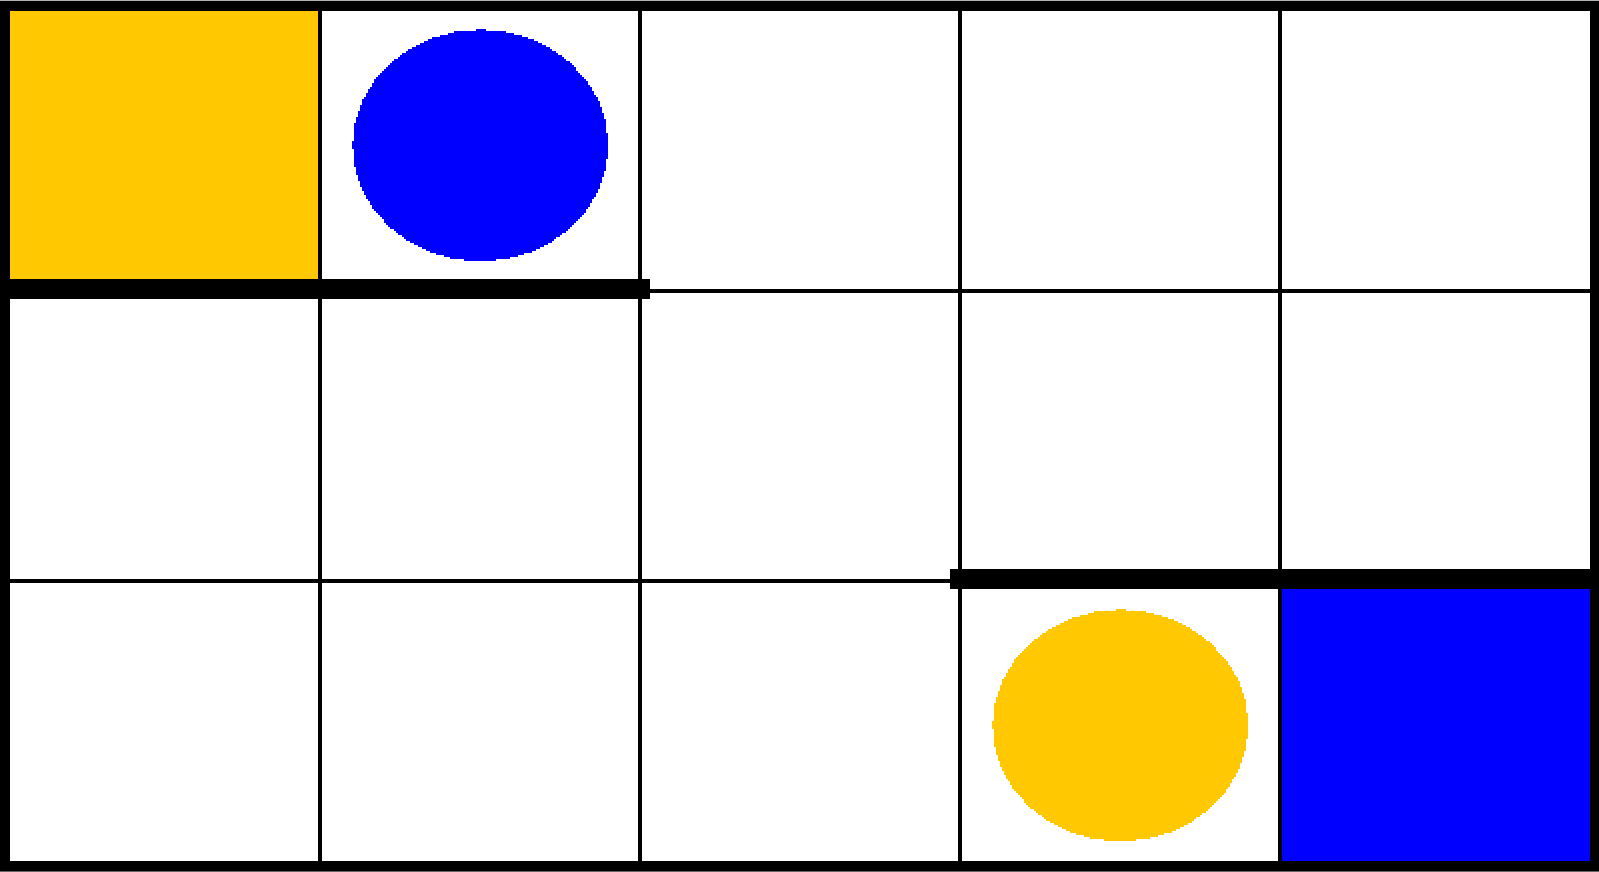
\includegraphics[width=0.65\columnwidth]{figures/threebyfivewindow.png}
%\caption{Door, a three-by-five grid that requires the partners to agree on an order in which to navigate through the center cell.}
\caption{Door}
\label{fig:door}
\end{subfigure} \\ [2.5ex]
\begin{subfigure}{.367\textwidth}
\centering
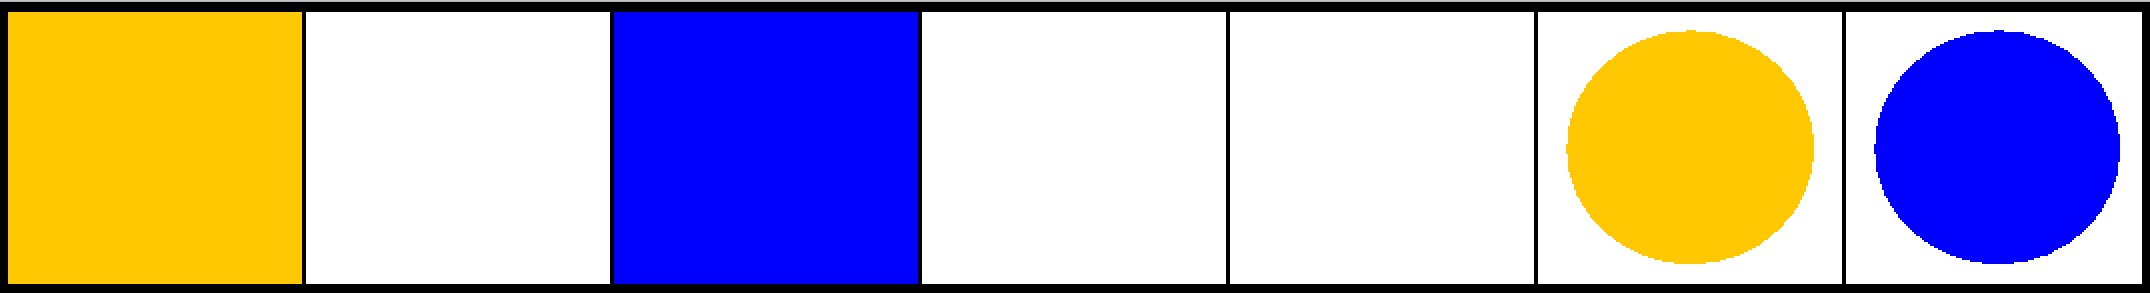
\includegraphics[width=0.5\columnwidth]{figures/longhallway.png}
\caption{Long Hall}
%\caption{Long Hall, a one-by-seven grid that allows Orange to squat on Blue's goal should they choose to not cooperate.}
\label{fig:longhallway}
\end{subfigure}
\begin{subfigure}{.367\textwidth}
\centering
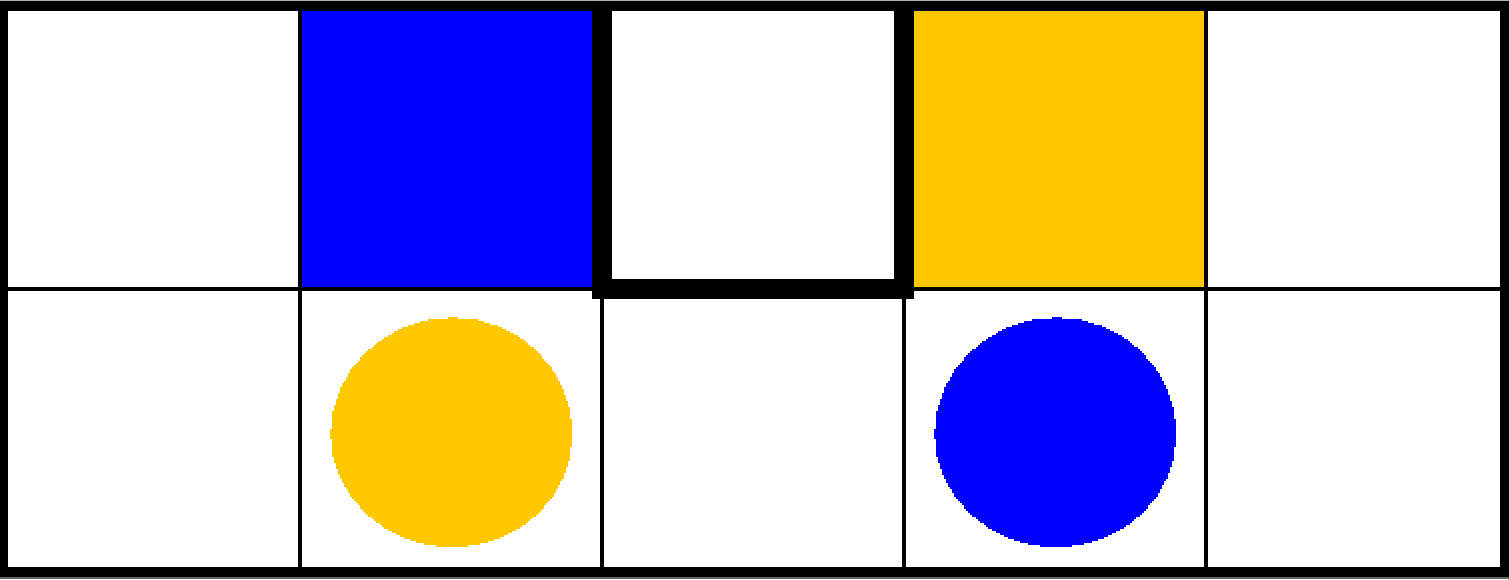
\includegraphics[width=0.5\columnwidth]{figures/nocompromise.png}
\caption{No Compromise}
%\caption{No Compromise, a two-by-five grid that requires one agent to sit on the other's goal and allow the other agent to pass, before it can move to its own goal.}
\label{fig:nocompromise}
\end{subfigure}
\caption{Five example grid games.}
\end{figure}

The grid in Figure~\ref{fig:intersection} (Intersection) requires Blue
to defend against the possibility of Orange behaving uncooperatively,
which it can achieve by squatting on the orange goal.  Orange can then
move to $(3,1)$ where both agents are equidistant from their goals.
Therefore, this game also has an equilibrium comprised of CD strategies
for both players.  

This equilibrium is not the shortest path, however.
%
Purely cooperative agents in this game could adopt a joint strategy in
which Blue moves east, while Orange waits a single step, before both
agents proceed into their goals.  This strategy profile is not
defensive for Blue though, because it does not have the opportunity to
observe if Orange will cooperate (wait) or defect (go north), and
therefore cannot defend itself if Orange decides to head straight
toward its goal.

%However, it is CD as both players are able to reach a position in
%which they are three turns from their goal without ever letting the
%other agent get closer than it is.

Figure~\ref{fig:door} (Door) is a grid that requires coordination to
navigate through the narrow center space at $(3,2)$. Any
equilibrium comprised of CD strategies for this grid must be asymmetric,
because it requires one agent to cede to the other agent the center
cell. For example, if Orange chooses to cede that cell, it should step
west into $(2,3)$ while Blue steps south into $(3,2)$. Then, Orange
needs to step east back into $(3,3)$ to prevent Blue from marching
straight into its goal. Only when Blue agrees to step aside to $(2,2)$
will they both be equidistant from their respective goals and in
position to cooperate.
%
This intricate pattern of first giving way to the opponent, and then
forcing them to step around later represents an equilibrium comprised
of CD strategies, since both agents are able to prohibit their
opponent from reaching the goal first, but still leaves open the
possibility for them both to reach their goals, cooperatively.

In the grid in Figure~\ref{fig:longhallway} (Long hall), Blue begins
one step closer to its goal than Orange does.  However, Orange can
squat on the blue goal until Blue chooses to cooperate by taking one
step back. If Orange can predict when Blue steps back, then Orange can
take one step closer to its goal while Blue steps further away, in
which case only Orange would reach its goal.  The strategy that
minimizes the risk to either agent requires that Blue wait one turn
initially, while Orange moves toward its goal.  These two strategies
comprise a CD equilibrium.

Our last grid, shown in Figure~\ref{fig:nocompromise} (No compromise),
requires not only cooperation, but both agents must also exhibit trust
for one another, or both agents cannot arrive at their goals at the
same time.  For example, Orange may sit on Blue's goal so that Blue
can move to $(1,2)$.  Then, Blue must wait two turns before both
agents are equidistant from the goals.  If Blue defects and moves
south into $(1,1)$ while Orange moves south into $(2,2)$, Orange still
has the opportunity to go back up north to block Blue from reaching
its goal.  However, if Blue moves south into $(1,1)$ when Orange steps
east into $(3,2)$, Blue will arrive at its goal sooner.  Therefore, a
trust spanning multiple rounds is required for the agents to
effectively cooperate in this game.

No equilibrium in CD strategies exists for No Compromise.  The game
is like Door in that only one player can go move through the middle
cell at a time.  Unlike Door, however, it is not possible for the
agents to simultaneously maintain a defensive position and to signal
cooperation, because any cooperative move leads to an asymmetric
situation in which the agents are no longer equidistant from their
goals.
%In other words, there's no way for one agent to signal cooperation by yielding the middle cell to the other, and then for the other agent to acknowledge that signal by moving to a position as far away from its goal as the first agent.
As a result, after one agent cooperates, there is always an incentive
for the other agent to defect, and there is nothing the cooperative
agent can do to defend itself.  Note however, that if Orange sits on
the blue goal while Blue walks to $(1,1)$ and then Blue cooperates by
waiting for Orange to walk to $(1,3)$, Blue's policy is CD.  Still,
Orange cannot respond in kind with a CD strategy; the aforementioned
strategy is C.

Taking these five grid games as an initial testbed, we performed two
pilot studies: the first involved simulations of artificial agents
playing against one another; the second pitted humans against other
humans on Mechanical Turk.  We report on the results of these
preliminary studies in the next two sections.  
%
%The main takeaway message of these experiments is that the behavior of
%both machines and humans can be at least partially explained as
%goal-driven.  In machines, those goals can be programmed directly via
%utility functions.  In humans, goals can be suggested, but the exact
%parameters governing a person's utility function are more difficult to
%control.  
%
The ultimate goal of this project, of course, is to design
artificial agents that play well with humans.  We propose to achieve
this goal by building agents that infer peoples' utility functions,
and then learn to collaborate appropriately based on these inferences.

